\section{Learning What Task Plan to Refine}
The approach presented thus far can be succinctly described as learning \emph{how} to
refine a single high-level plan. In this section, we present a method for learning
\emph{which} plan to try refining. Recall that in Alg.\,\ref{alg:complete}, the high
level has a two-tiered decision to make: which node in the {\sc prg} to
visit next, and whether to attempt to refine this node or generate failure information
from it. These decisions are encoded in the routines \textsc{NDGetNextNode}
and \textsc{NDChoice}. \figref{fig:cover} illustrates why making this decision intelligently is critical
to good performance (TODO: remove this). We now explain our inverse {\sc rl}
approach to training heuristics that implement these routines. The heuristics are trained to estimate
the difficulty associated with refining a plan, and to decide when to quickly generate
a geometric fact used for replanning with the task planner. In our explanation, $n$ is the selected
node and $m$ is the mode to apply (either trying to refine the node or quickly generating failure information).

We exploit properties of the environment to hand-design a feature vector $f(n)$ that encodes the refinability
of a single high-level plan. Because the mode $m$ is binary,
we construct $$f((n, m)) = \begin{bmatrix} f(n) \\ f(n) \end{bmatrix}^\top \begin{bmatrix} 1 - m \\ m \end{bmatrix},$$
which stacks the feature vector for $n$ on itself, then turns off the bottom half when $m = 0$ and the
top half when $m = 1$. Now that we have defined a feature vector associated with each decision in a given {\sc prg},
we can obtain human-demonstrated trajectories (sequences of actions $(n, m)^{*}$) that intelligently
navigate the {\sc prg}. We then solve the following maximum-margin optimization problem with a constant margin and slack variables:
\begin{align*}
&\min_{w, \xi_i \geq 0} & ||w||^2 + C \sum_i \xi_i\\
&\text{s.t.} & w^{\top}f^*_i \geq w^{\top}f_{ij} + 1 - \xi_{i}\ \forall i, j \ ,
\end{align*}

where the $i$ iterate over the demonstrated trajectories and the $j$ iterate over possible actions. Each
demonstrated trajectory has an associated slack variable in this formulation.
The weight vector $w$ encodes a ranking function on the different actions.
We then use {\sc DAgger}~\cite{dagger} to augment our training data. At test time, we follow the policy encoded by
$w$, picking the highest-scoring action at each step.

TODO: cite \figref{fig:hlsearch}

\begin{figure}[t]
  \centering
    \noindent
    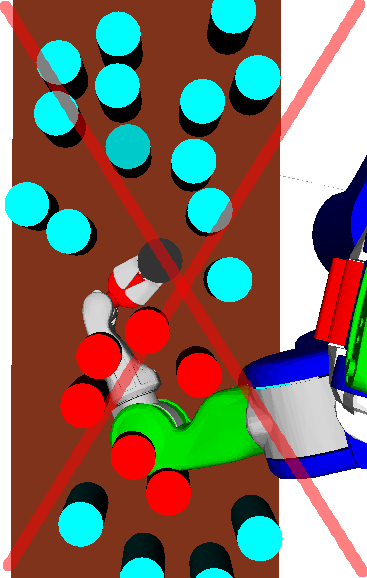
\includegraphics[scale=0.17, angle=270]{images/grasp_teaser_bad.png}
    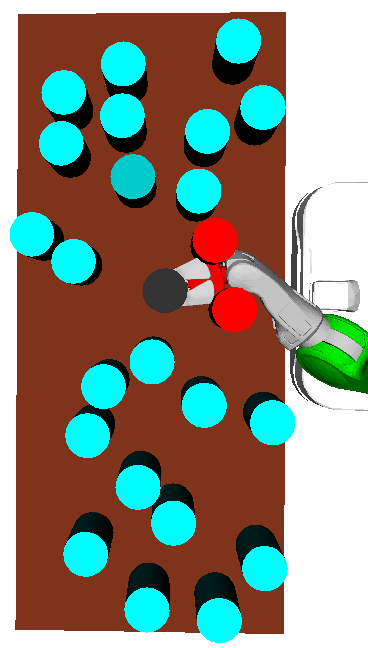
\includegraphics[scale=0.17, angle=270]{images/grasp_teaser_good.png}
  \caption{\small{When trying to grasp the black can, the sampled grasping pose can
      significantly affect the quality of the obstructions determined. The new plan proposed from the rightmost image only
      requires moving 2 obstructions out of the way, versus 6 from the other. We integrate inverse reinforcement learning into our task and
      motion planning system to learn an ordering on plan exploration, causing the system to prefer simpler and more feasible plans.}}
  \label{fig:hlsearch}
\end{figure}

% \begin{figure}[t]
%   \centering
%     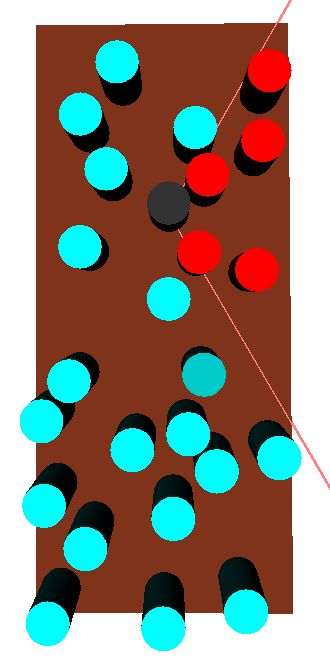
\includegraphics[scale=0.3,angle=90]{images/feature_cone.png}
%   \caption{\small{If the target object to be grasped is the black can, we consider the objects
% whose centers lie in a cone from angles $-\frac{\pi}{3}$ to $\frac{\pi}{3}$ toward the closest table edge in
% our feature computations. These objects are shown here in red.}}
%   \label{fig:cone}
% \end{figure}
